
The core calculus of NomosUC relies on \emph{import session types}, a novel derivative of
binary session types.
We will introduce this calculus in two phases.
In this section, we discuss the base system of session types, whereas the next section
will introduce the import annotations.
We note that some of the base system rules carry over from existing work by Das et al.~\cite{Das20FSCD}, and we add to them new features like the write token and import token typing rules in the following section. 
Session types are derived from a Curry-Howard interpretation of intuitionistic linear logic~\cite{girard1987linear}.
Under this correspondence, a process term $P$ is assigned the following typing judgment
\[
(x_1 : A_1), (x_2 : A_2), \ldots, (x_n : A_n) \vdash P :: (z : C)
\]
which states that process $P$ \emph{provides} a service
of session type $C$ along channel $z$, \emph{using} the services of session
types $A_1, \ldots, A_n$ provided along channels $x_1, \ldots, x_n$ respectively.
For a \emph{well-formed} judgment, all channel names need to be distinct.
The linear antecedents are often abbreviated to $\D$.
The sender and receiver channels are the antecedents of \Fcom in Figure~\ref{fig:fcomideal}(b) 
and its offered channel \inline{fc} unused.
In general throughout this work we don't use the offered channels of processes 
aside from the \emph{providerless channels} which we discuss in detail later in this
section. 

The NomosUC judgment has some additional components
\[
\Sg \semi k \semi \Tokens \semi \Psi \semi \D \entailpot{q}{q'} P :: (x : A)
\]

$\Sg$ denotes the signature containing type and process definitions and $k$
denotes the security parameter.
Both these quantities are globally known and fixed, therefore we omit them from
most typing rules for brevity.
$\Tokens$ describes the total (ever received) and current ($=$ received - sent) import tokens
of each type stored in the process (explained more in Section~\ref{sec:import}).
$\Psi$ represents the functional data structures and $\D$ collects the
session-typed channels along with an optional \emph{write token} $\wt$
(to resolve non-determinism in the semantics) used by the process.
Intuitively, the sender must possess the write token before it can 
send a commitment to \Fcom. The token is transferred to \Fcom which then 
gives it to the receiver along with the \m{Commit} message.
%Intuitively, the process sending a message \emph{must possess} the write
%token which is then transferred to the receiver along with the message.
Globally, the process owning the write token is activated to take the
next execution step.
%Finally, $P$ is the process expression that is currently being executed and
%the process offers channel $x$ of type $A$.
Similar to import tokens, the natural number annotations $q$ and $q'$ on the turnstile
denote the total and current potential stored in the process.
We will gradually explain each component of the language, initiating
with the basic system of session types.
For simplicity of exposition, we will mark the yet unexplained
parts of the system in \B{gray}.

The operational semantics of NomosUC is formalized as a
system of \emph{multiset rewriting rules}~\cite{cervesato2009relating}.
These rules consist of semantic objects $\proc{c}{w, P}$ and $\msg{c}{w, M}$ describing
process $P$ (or message $M$) providing service along channel $c$.
The work counter $w$ stores the work performed
(number of computational steps executed) by process $P$ (resp. message $M$).
Remarkably, in this formulation, a message is just a particular form of process,
thereby not requiring any special rules for typing; it can be typed just as processes.

\subsection{Session Type Constructors}
\label{subsec:constructors}
NomosUC uses only a subset of session type constructors since we did not find
any application of exchanging channels over channels in UC experiments.
We briefly describe a representative set of these session-typed constructors
with full details in Appendix~\ref{app:typing_rules}.

\paragraph*{\textbf{Choice Operators}}
The choice operators are used by processes to send messages over channels,
formally.
The internal choice $\ichoice{\ell : A_\ell}_{\ell \in L}$ constructor
is an $n$-ary labeled generalization of the additive disjunction $A \oplus B$.
A process that provides  $x : \ichoice{\ell : A_\ell}_{\ell \in L}$ can send
any label $l \in L$ along $x$ and then continue by providing $x : A_l$. 
The sender in \Fcom is the provider and has one label to chose from: \m{Commit}.
The channel then transitions to a new type whose only available label is \m{Open}.
%The corresponding process is written as $(\esendl{x}{l} \semi P)$, where
%$P$ is the continuation that provides $A_l$.
On the other end of the channel, the client \Fcom branches on the label received along $x$.
The provider and client are typed according to the following $\oplus R$ and $\oplus L$
rules, respectively (we omit $\Sg, k, \Psi, \Tokens$ from the rules since they are constants).
Additionally, the provider should possess the write token to be able to send the
label. Dually, the client receives the write token with the label to continue
execution.
\begin{mathpar} \small
  \infer[{\oplus}R]
  {\wt, \D \entailpot{\B{q}}{\B{q'}} (\esendl{x}{l} \semi P) ::
    (x : \ichoice{\ell : A_\ell}_{\ell \in L})}
  {(l \in L) \qquad \D \entailpot{\B{q}}{\B{q'}} P :: (x : A_l)}
\end{mathpar}
\begin{mathpar}
  \infer[{\oplus}L]
  {\D, (x : \ichoice{\ell : A_\ell}_{\ell \in L})
    \entailpot{\B{q}}{\B{q'}} \ecase{x}{\ell}{Q_\ell}_{\ell \in L} :: (z : C)}
  {(\forall \ell \in L) \qquad \wt, \D, (x : A_\ell)
    \entailpot{\B{q}}{\B{q'}} Q_\ell :: (z : C)}
\end{mathpar}

\paragraph{Message Ordering}
Communication in NomosUC is asynchronous, and the process $P$ sends a message $l$
along $c$ and continues as $P$ substituting $c$ for a new channel $c'$. Creating a new
channel $c'$ ensures that messages arrive in order. 
Naturally, a message send doesn't consume work ($q,q'$) but, as we'll see later, can 
transfer import between processes. 
%Operationally, since communication is asynchronous, the process
%$(\esendl{c}{l} \semi P)$ sends a message $l$
%along $c$ and continues as $P$ without waiting for it to be received.
%As a technical device to ensure that consecutive messages on a
%channel arrive in order, the sender also creates a fresh continuation
%channel $c'$ so that the message $k$ is actually represented as
%$(\esendl{c}{l} \semi \fwd{c}{c'})$ (read: send $l$ along $c$ and
%continue as $c'$). The provider substitutes $c'$ for $c$ enforcing
%that the next message is sent on $c'$.
%The work counter of the process remains unaltered, and the new message
%is created with work $0$.
%\begin{tabbing}
%$(\oplus S) : \proc{c}{w, \esendl{c}{l} \semi P} \step$ \\
%\qquad $\proc{c'}{w, [c'/c]P},
%\msg{c}{0, \esendl{c}{l} \semi \fwd{c}{c'}} \qquad \fresh{c'}$
%\end{tabbing}
When the message $l$ is received along $c$, the client selects branch
$l$ and also substitutes the continuation channel $c'$ for $c$, thereby
ensuring that it receives the next message on $c'$. This implicit
substitution of the continuation channel ensures the ordering of the
messages.
The client process also collects the work performed by the message, if
there is any.
%\begin{tabbing}
%$(\oplus C) :$ \= $\msg{c}{w, \esendl{c}{l} \semi \fwd{c}{c'}},
%\proc{d}{w', \ecase{c}{\ell}{Q_\ell}}$ \\
%$\qquad \qquad \step \proc{d}{w+w',[c'/c]Q_l}$
%\end{tabbing}

The dual of internal choice is \emph{external choice} $\echoice{\ell :
A_\ell}_{\ell \in L}$, which reverses the role of the provider and client.
The provider process of $x : \echoice{\ell : A_\ell}_{\ell \in L}$ branches on receiving a label
using the expression $\ecase{x}{\ell}{Q_\ell}_{\ell \in L}$,
while the client sends one such label in $L$.
\Fcom is the client for the channel with the receiver, and performs an external choice operation
when sending the label $\m{Committed}$ to the receiver.
% using the expression $(\esendl{x}{l} \semi P)$.
% $k \in L$ (described in $\with R$), while the client sends this label
% (described in $\with L$).
% \begin{mathpar}
%   \footnotesize
%   \infer[\with R]
%   {\B{k \semi \Tokens \semi \Psi} \semi \D \entailpot{\B{q}}{\B{q'}} \ecase{x}{\ell}{P_\ell}_{\ell \in L} ::
%     (x : \echoice{\ell : A_\ell}_{\ell \in L})}
%   {(\forall \ell \in L) \qquad \B{k \semi \Tokens \semi \Psi} \semi \wt, \D
%     \entailpot{\B{q}}{\B{q'}} P_\ell :: (x : A_\ell)}
% \end{mathpar}
% \begin{mathpar}
%   \footnotesize
%   \infer[\with L]
%   {\B{k \semi \Tokens \semi \Psi} \semi \wt, \D, (x : \echoice{\ell : A_\ell}_{\ell \in L})
%     \entailpot{\B{q}}{\B{q'}} \esendl{x}{k} \semi Q :: (z : C)}
%   {\B{k \semi \Tokens \semi \Psi} \semi \D, (x : A_k) \entailpot{\B{q}}{\B{q'}} Q :: (z : C)}
% \end{mathpar}
Dual to internal choice, the client \Fcom contains the write token which is
sent to the channel provider, the receiver in this case, along with the label.
The typing and semantics rules for external choice are just the inverse of internal choice,
and presented in Appendix~\ref{app:typing_rules}.

% \paragraph*{\textbf{Termination}}
% The type $\one$, the multiplicative unit of linear logic, represents
% termination of a process, which is not allowed to use
% any linear channels. A terminating process offering on $x : \one$ simply
% closes channel $x$ using the expression $\eclose{x}$ while the client waits
% for this close message to arrive using the expression $\ewait{x} \semi Q$
% and then continues executing $Q$.
% The typing rules are presented in Appendix~\ref{app:typing_rules}.
% Operationally, the provider converts into a closing message
% with no continuation since the offered channel terminates.
% \begin{tabbing}
% $(\one S) : \proc{c}{\eclose{c}} \step \msg{c}{\eclose{c}}$ \\
% $(\one C) : \msg{c}{\eclose{c}}, \proc{d}{\ewait{c} \semi Q} \step
% \proc{d}{Q}$
% \end{tabbing}

% The provider receives the branching label $k$ sent by the provider. Both
% processes perform appropriate substitutions to ensure the order of messages
% sent and received is preserved.
% \[
% \begin{array}{lll}
% (\with S) & \proc{d}{\esendl{c}{k} \semi Q} \step \msg{c'}{\esendl{c}{k}
% \semi \fwd{c'}{c}}, \proc{d}{[c'/c]Q} & \fresh{c'} \\
% (\with C) & \proc{c}{\ecase{c}{\ell}{Q_\ell}_{\ell \in L}},
% \msg{c'}{\esendl{c}{k} \semi \fwd{c'}{c}} \step \proc{c'}{[c'/c]Q_k}
% \end{array}
% \]

\paragraph*{\textbf{Exchanging Functional Data}}
We now turn our attention to the functional layer $\Psi$ that contains the
traditional data structures and values.
Communicating a \emph{value} of the functional fragment along a channel
is expressed at the type level by adding the following two session types.
\begin{center}
\begin{minipage}{0cm}
\begin{tabbing}
$A ::= \ldots \mid \tau \arrow A \mid \tau \product A$
\end{tabbing}
\end{minipage}
\end{center}
Here, $\tau$ describes a functional type, e.g. $\m{int}, \m{bool}, \tau \; \m{list}$, etc
(we assume the language contains standard functional types).
The type $\tau \arrow A$ prescribes receiving a value of type $\tau$
with continuation type $A$, while its dual $\tau \product A$ prescribes
sending a value of type $\tau$ with continuation $A$. The corresponding
typing rules for arrow ($\arrow R, \arrow L$) are given in Appendix~\ref{app:typing_rules}.
The $\product$ operator is dual to $\arrow$ reversing the roles of provider and client,
and we omit its explanation for brevity.

\subsection{Cyclic Communication via Shared Session Types}
\label{subsec:communicators}
%Despite the seemingly structured nature of execution in UC, the framework is meant to
%capture arbitrary connections, communication patterns, or configurations of ITMs.
%However, linear session types can prove to be quite restrictive in terms of realizing
%arbitrary communication patterns in practical cryptographic protocols.
%In this section, we highlight a common communication pattern in UC that requires introducing
%the notion of shared session types~\cite{balzer2017manifest} to be expressible in NomosUC.

% Consider two ITMs $P$ and $Q$ that communicate in the following way. If $P$ is activated first,
% it sends a message to $Q$ and terminates, but if $Q$ is activated first it writes a message to $P$, 
% $P$ writes a message back, and communication terminates.
% Session types require it to be statically known which party will write next to a channel so such
% a communication pattern can not be realized by juts a single session type.

% If we try to resolve this by splitting communication among two channels, we may type them as
% %\begin{center}
% \vspace{2mm}

% {\centering
%  $\m{PtoQ} = \ichoice{\mb{one}: int \tensor 1}$ \\
%  $\m{QtoP} = \echoice{\mb{one}: int \tensor \ichoice{\mb{end}: int \tensor 1}}$
% %\end{center}
% \par}
% \vspace{2mm}

We want to realize arbitrary ITM topologies in NomosUC but the session type constructors we discussed so far are \emph{linear} and impose a tree-like topology
on the process network.
This topology is enforced because session-typed channels create a \emph{parent-child relationship} among processes
where the client of a channel is the parent, while the provider is the child.
%We can imagine every process in a tree configuration, where it is connected to its parent via its provided channel,
%and connected to its (possibly multiple) children via its client channels.
These endpoints are fixed, i.e., a process cannot transition from being a client of
a channel to its provider, or vice-versa.
This means that even simple configurations in UC can't be realized directly with session types.
For example, imagine a simple UC executing with an environment \Z, two parties $P_1$ and $P_2$, and some ideal functionality \F.
We would expect a channel between \Z and each of $P_1$/$P_2$, and a channel between \F and each of $P_1$/$P_2$. 
If we rely purely on offered linear channels, one of the four connections we want can not exist, as it would require one provided channel to have two clients. 

%Unfortunately, this places a strong restriction on the expressiveness of the language and precludes practical
%programming scenarios where a cyclic topology is required.
UC places no such restriction on ITMs, which can arbitrarily communicate with each other, even in a cycle.
% If $P$ and $Q$ connected by two channels creates ambiguity between their parent child relationship: a cycle. One processes must have spawned the other. 
% In general, this restriction results in an acyclic tree-like topology among processes where parents progressively
% spawn child processes becoming the client to the channel provided by the child.
%On the other hand, UC places no such restriction on communication and cyclic communication
%is quite common in UC protocols.
Thus, a direct translation from ITM terms to NomosUC expressions can result in cyclic
dependency among channels, thus causing the program to be ill-typed.

% The pattern emerges from the following code: a machine $P$ either writes to another machine $Q$ or is written to by $Q$. 
% At first glance, it is a trivial scenario, but we encounter a problem trying to encode this with a single session type.
% A example are machines $P$ and $Q$ which execute as follows:
% \begin{itemize}
% 	\item An external machines flips a bit and activates either $P$ or $Q$.
% 	\item If $P$ is activated it writes to $Q$ and the execution terminates. 
% 	\item Otherwise, if $Q$ is activated, it writes a message to $P$, $P$ writes something back, and the execution terminates.
% \end{itemize}
% A single type between $P$ and $Q$ would have to allow either of the two parties to write on the channel, but session types require it to be statically known.
%
% If we try to separate communication between $P$ and $Q$ into two uni-directional channel, we can express the session type for each of the channels:
% \begin{center}
% \parbox{0cm}{
% \begin{tabbing}
% $\m{PtoQ} = \ichoice{\mb{``one''}: int \tensor 1}$ \\
% $\m{QtoP} = \echoice{\mb{``one''}: int \tensor \ichoice{\mb{``end''}: int \tensor 1}}$
% \end{tabbing}}
% \end{center}
%
% This approach, however, poses another problem. 
% Channels are only created by a process offering them, and a process can only offer a single channel.
% Without adding any additional processes, $P$ must offer a channel to $Q$ and $Q$ offer one to $P$. 
% Each of them becomes both a provider and a client to the other, and provider/client ambiguity is not allowed in Nomos. 
% Logically, one process must have spawned the other, and such a cycle would be impossible to realize.

To enable arbitrary communication between two processes without forcing a parent-child relationship, we introduce
the concept of \emph{providerless channels} using \emph{communicator processes} that rely on recently introduced shared session types~\cite{balzer2017manifest}.
Communicators act as a buffer between two processes allowing them to exchange messages via the communicator.
Communicators also break the parent-child relationship by offering a \emph{shared channel that can have multiple clients}
(unlike linear channels that can have only one client) that is then used by both the sender and receiver processes.

The communicator has the following polymorphic type:
%\begin{center}

\vspace{-1mm}
{\centering
\parbox{0cm}{
\begin{tabbing}
$\m{comm[\tau]\{n\}} = \up \echoice{$\=$ \textcolor{red}{\getpot^n} \mb{push}: \m{\tau} \arrow \m \down \m{comm[\tau]},$\\
\>$\textcolor{red}{\getpot^0} \mb{poll}: \ichoice{$\=$\textcolor{red}{\paypot^{n-1}} \mb{yes}: \m{\tau} \;\product \down \m{comm[\tau]},$\\
\>\>$\textcolor{red}{\paypot^0} \mb{no}: \; \down \m{comm[\tau]}}}$
\end{tabbing}}
%\end{center}
\par}

The communicator type uses the type constructions $\up$ and $\down$ to indicate that 
access to the channel must be \emph{acquired} and eventually \emph{released}, respectively.
The acquire-release paradigm, along with the write token, is necessary for shared session types to prevent non-determinism.
Communicators are written to by a sender that acquires the channel and $\mb{push}$es a functionally 
typed message along with some amount of import indicated as a parameter. A receiver acquires the 
channels and asks the communicator for new messages with $\mb{poll}$ if there is a message it is returned with some import
otherwise the channels takes the $\mb{no}$ branch.
We provide the full typing rule of shared session types in Appendix~\ref{app:typing_rules}.

%The communicator type relies on shared type constructors $\up$ and $\down$.
%The type initiates with an $\up$ indicating that the communicator channel must be \emph{acquired} to interact with it.
%Because the channel has two clients (the sender and the receiver), either of them can acquire this channel
%but in mutual exclusion, i.e., they both cannot acquire the channel simultaneously.
%The sender only interacts with the communicator on the $\mb{push}$ branch, while the receiver only uses
%the $\mb{poll}$ branch.
%Once acquired, the sender sends $\mb{push}$ along with the actual message of type $\tau$ and some amoutn of import tokens $n$. 
%On the other hand, the receiver, after the acquire, sends the $\mb{poll}$ message and gets a $\mb{yes}$ 
%or $\mb{no}$ reply depending on whether there is a pending message for it.
%If yes, the receiver gets the message of type $\tau$ using the $\times$ constructor with the import tokens accompanying the message, otherwise it gets nothing.
%Then, in all cases, the type transitions to $\down$, meaning the sender (or receiver) \emph{release} the acquired
%channel detaching from the communicator.
%% Then the sender releases the channel so that the receiver can interact with the communicator and check, with $\mb{RECV}$ whether 
%% there is a message waiting or not.
%We provide the full typing rule of shared session types in Appendix~\ref{app:typing_rules}.
%Then, the type transitions to $\down$ meaning that the sender sends a \emph{release} request to the communicator effectively
%detaching from it so that the receiver can interact with the communicator.
%In the latter case, the communicator gets the $\mb{RECV}$ request from the receiver and checks whether the there is a message
%waiting for the receiver or not.
%If a message is found, the communicator replies with a $\mb{yes}$ message followed by the message of type $\tau$, and if not,
%the $\mb{no}$ message is sent.
%Finally, in either case, the communicator detaches from the receiver as indicated by the $\down$ constructor.

%Shared session types impose an \emph{acquire-release} discipline on processes; 
%a client must acquire the channel offered by a shared process to interact with it
%and must release this channel after the interaction.
%The corresponding typing rules are
%\begin{mathpar}
%  \infer[\up L]
%  {\Tokens \semi \Psi \semi \wt, \D, (x : \up A_L)
%  \entailpot{q}{q'} \eacquire{y}{x} \semi Q :: (z : C)}
%  {\Tokens \semi \Psi \semi \D, (y : A_L)
%  \entailpot{q}{q'} Q :: (z : C)}
%  %
%  \and
%  %
%  \infer[\up R]
%  {\Tokens \semi \Psi \semi \D \entailpot{q}{q'}
%  \eaccept{y}{x} \semi P :: (x : \up A_L)}
%  {\Tokens \semi \Psi \semi \wt, \D \entailpot{q}{q'} P :: (y : A_L)}
%\end{mathpar}
%The $\up L$ rule describes a client acquiring a shared channel $x$
%and obtaining a private linear channel $y$ along which it can communicate
%with the corresponding acquired process.
%Correspondingly, the $\up R$ rule describes the shared process
%accepting the acquire request and creating the fresh linear channel $y$.
%The release-detach rules corresponding to the $\down$ type constructor
%are exact dual of acquire-accept.

%An important caveat here is that shared channels can introduce non-determinism
%in the semantics since the communicator can accept an acquire request from
%either the sender or the receiver.
%Fortunately, the \emph{write token} resolves this non-determinism and we require that
%the acquiring process must possess the write token.
%This resolves both read and write non-determinism due to linearity of the channels.

%An essential constraint for shared types to be type-safe is that they must be acquired
%and released at the \emph{same} type (in our case $\m{comm}[\tau]$).
%Therefore, communicators lose the \emph{order} in which messages are exchanged
%between two processes since they keep recursing back to the same type after each interaction.
%For instance, consider processes $P$ and $Q$ such that $P$ sends an integer, then a boolean to $Q$,
%and terminates, expressed by the type $\m{PtoQ} = \m{int} \product \m{bool} \product \one$
%The corresponding commuicator type for this exchange is $\m{comm[\tau_{\m{PtoQ}}]}$
%where $\tau_{\m{PtoQ}} = \m{int} \lor \m{bool}$, forgetting $\m{int}$ is sent
%before $\m{bool}$.

A major constraint of communicators is that the $\tau$ parameter in their type is a functional type
and not a session type. This means that even if we can realize cyclic topologies, we lose the protocol and message ordering
that session types give us. 
For example, in place of channels typed with \m{receiver} or \m{sender} from the commitment example, communicator channels would be typed \m{comm}[\m{sender2f}], where 
\inline{type  sender2f = Commit of Bit | Open},
resembling a typical functional data type.
It's obvious here that the ordering of messages that \m{sender} provided is lost with the communicator.
We overcome this constraint by abstracting channels in NomosUC into higher-level constructs called \emph{providerless channels}.
First, we wrap processes in shell code that creates dummy intermediaries ($a_Q$ and $a_P$ in Figure~\ref{fig:newpandq}) which
create channels with the desired session type (for example \m{sender} in the case of \Fcom). The shell processes, however, still communicate through communicators without ordering. 
The shell code relies on processes $a_P$ and $a_Q$ (and $b_Q$ and $b_P$) to convert messages from the session types to 
functionally types messages that the communicators can accept, and vice versa.

%How can we use shared communicators to enable cyclic topologies while retaining the ordering
%of message exchanges that are the crux behind session types?
%We address this by introducing a novel channel abstraction called \emph{providerless channels}.
%Refer to Figure~\ref{fig:pandq} where we have two distinct channels with their corresponding
%session type.
%To break the parent-child asymmetry while retaining  the message orderings, we introduce
%intermediate processes $a_P$ and $a_Q$ (Figure~\ref{fig:newpandq}). The process $a_P$ converts
%messages from type $\m{PtoQ}$ to $\m{comm[\tau_{PtoQ}]}$.
%Then, $C$ acts as the shared communicator between $a_P$ and $a_Q$.
%Finally, $a_Q$ converts messages from $\m{comm[\tau_{PtoQ}]}$ back to type $\m{PtoQ}$, as desired.
%Processes $b_P$ and $b_Q$ achieve the same result for $\m{QtoP}$.
% that combines communicators with processes that offer the linear session type desired. 
% Take, for example, Figure~\ref{fig:newpandq}. Here we wish to realize communication with the session types mentioned previously: \m{PtoQ} and \m{QtoP}.
% We begin by running the process $P$ in a wrapper that manages its communication.
% For each session type, in this case 2, the wrapper spawns a generated process, $a_p$ and $b_p$ in the diagram, which offer the session types \m{PtoQ} and \m{QtoP}. The wrapper connects to the communicators.
% Providerless channels allow the process $P$, and $Q$ respectively, to communicate only over desired session types, and they abstract away communicators alltogether. 
An important note to providerless channels are that processes $a_P$, $a_Q$, $b_P$, and $b_Q$ can be defined
generically if the types $\m{PtoQ}$ and $\m{QtoP}$ are known.
Typically, such protocol-specific communication constructs are written by users, as is the case with the addressing scheme in EasyUC~\cite{easyuc},
but in NomosUC the processes themselves are so trivial that they can be generated automatically.
We call this intermediate sub-configuration as \emph{communicator wrapper} (box in Figure~\ref{fig:newpandq}).

%The final constraint imposed by communicators is that the type $\m{comm[\tau]}$ forces a constant amount of import to be sent over it with every message.
%Although this may restrict expressiveness of tight runtime bounds, generally, we care more about amount of net import a process has rather than how much is sent wit each message.
%We do not see this as a downside of the approach, however, as tight runtime constraints are not an intended goal of NomosUC or the UC framework. 

%Finally, in order to send import over the communicator, its type $\msf{comm[\tau]}$ is restricted to a constant amount of import received on \m{push} and sent out on \m{yes}.
%Regardless of what import is required by the channel offered by, say, $\m{a_P}$, the communicator \m{c} connecting it to $\m{a_Q}$ must accept and send at least the maximum import required by any type originating from $\m{PtoQ}$.
%For example if $\m{PtoQ}$ sometimes sends 1 to $Q$ import on every message and $\m{QtoP}$ sends 1 import $P$ only once, $Q$ ends up with a positive import balance.
%The constant import requirement for providerless channels would require at least 1 import to be sent with every message in both directions, leading to net 0 import for both. 
%Therefore, when assigning import values to session types, requires careful consideration to ensure each process ends up with enough import at the end of its activation. 
%Finally, to bound the execution time of these communicator wrappers, we require at most a constant amount of import sent over them with each message.
%This is because at each activation, these intermediate processes do a constant amount of work to convert messages from one type to another. 
% The virtual channels and process still receive virtual tokens according to their session type. 
%Each shell spawns two processes, call then $a$ and $b$, which offer the types \m{PtoQ} and \m{Qto} to each of $P$ and $Q$. They also handle functional messages from the communicators and sends the corresponding message, specified by the session type, on the channels they offer. %\snote{Cleared up this point, the previous one and your comment is commented out in the latex.}
%%The two processes, call them $a$ and $b$, perform two tasks. First $a$ and $b$ offer, say to $P$, the desired session types of \m{PtoQ} and \m{QtoP}.\anote{This is an awkward explanation, more iteration to make it simpler would help}
%%Second, $a$ and $b$ each communicate with one communicator and convert functionally typed messages received from them to ones that are send along their session typed channels to $P$ (and vice versa).
%Although the process code for terms $a$ and $b$ differ based on the session type being used, they can be systematically generated as a case switch between functional and session typed messages.
\begin{figure}
	\begin{subfigure}{0.5\textwidth}
	\begin{center}
	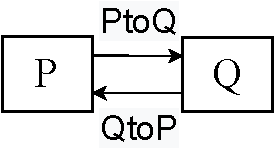
\includegraphics[scale=0.5]{figures/p_and_q.pdf}
	\caption{Goal: $P$, $Q$ connected by channels labeled with their types.}
	\label{fig:pandq}
	\end{center}
	\vspace{0.1em}
	\end{subfigure}
	\begin{subfigure}{0.5\textwidth}
	\begin{center}
	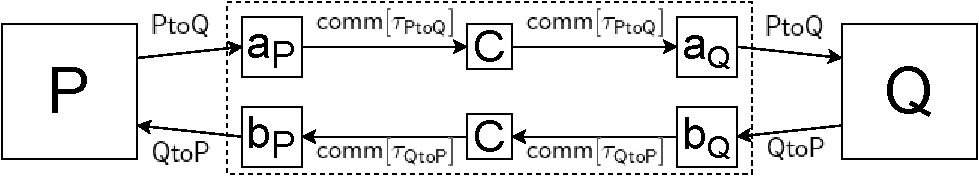
\includegraphics[scale=0.4]{figures/newPandQ.pdf}
	\caption{Internal implementation of channels using communication\\wrapper
	with channels labeled with their session types.}
	\label{fig:newpandq}
	\end{center}
	\end{subfigure}
	\caption{Two ITM configurations. One possible with ITMs (top) and one realized in NomosUC (bottom). Arrows indicate direction of messages
	and labels indicate types.}
	\vspace{-1em}
\end{figure}

% Splitting communication over two channels in this way also imposes constraints on the expressiveness of session types. 
% An example of the motivating case is a two-way communication channel \Fauth.
% \Fauth accepts messages from two parties and allows \A to decide when the message is delivered to the other.
% At a given moment, party $P_i$ can give input to, or expect output from, \Fauth. This implies a session type must both accept internal choice and external choice at the same time---a pattern that can not be realized.
% Splitting communication into two uni-directional channels like the $P$ and $Q$ example results in the following session type:
% \begin{center}
% \parbox{0cm}{
% \begin{tabbing}
% $\m{sendmsg}[a] = \textcolor{red}{\getpot^n} \ichoice{\mb{send}: \m{a} \product \m{sendmsg}}$ \\
% $\m{recvmsg}[a] = \textcolor{red}{\getpot^m} \echoice{\mb{recv}: \m{a} \product \m{recvmsg}}$ \\
% $\m{adv}[a] = \echoice{\mb{leakmsg}: a \product \ichoice{ \mb{ok}: \m{adv}}}$
% \end{tabbing}}
% \end{center}
% The intended ordering of a send before a read is lost by splitting the session type like this, however we can recover some expressiveness by making use of polymorphism in our types. In this example the session types are parameterized by a type \inline{a}. 
% Only the sender of the message can concretize the parameter \inline{a} forcing \Fauth to wait for a message send before giving a message to the receiver. 
% In general, this trick can be used to enforce an ordering of messages between different channels.

% From now on we only discuss communication in the form of session types and providerless channels.
% We encounter an example of shared channels and creating a providerless channel in Section~\ref{sec:commitment}.

